\chapter{Inference using linear models}
\label{sec_inf_lin_mods}
In this chapter we consider probabilistic graphical models of the form shown in figure~\ref{fig_linmod2}. This model is a generalisation of the graphical model seen in chapter \ref{sec_hmm}. We now assume that the states ($x_0,x_1,x_2,\hdots$) and observations ($y_0,y_1,y_2,\hdots$) are continuous random variables but the inputs ($u_0,u_1,u_2,\hdots$) are continuous deterministic variables. Models of this form are called latent dynamical systems - if one assumes linearity and normality the famous Kalman filter model falls into this category.
\begin{figure}[H] 
\centering
\begin{tikzpicture}

  % Define nodes
  \node[obs] (ya) {$y_0$};
  \node[obs, right=of ya] (yb) {$y_1$};
  \node[obs, right=of yb] (yc) {$y_2$};
  \node[latent, above=of ya]  (xa) {$x_0$};
  \node[latent, above=of yb, right=of xa]  (xb) {$x_1$};
  \node[latent, above=of yc, right=of xb]  (xc) {$x_2$};
  \node[det, above=of xa] (da) {$u_0$};
  \node[det, above=of xb] (db) {$u_1$};
  
  % Connect the nodes
  \edge {da} {xb};
  \edge {db} {xc};
  \edge {xa} {ya};
  \edge {xb} {yb};
  \edge {xc} {yc};
  \edge {xa} {xb};
  \edge {xb} {xc};
  
\end{tikzpicture}
\caption{Graphical model considered in this chapter.}
\label{fig_linmod2}
\end{figure}
In chapter \ref{sec_hmm} we developed inference algorithms but assumed that the transition and observation functions were discrete. We also noted that this assumption is not appropriate for continuous systems. The reason is that one would invariably need to discretise the domain of the continuous random variable under consideration. This would result in intractably large discrete systems if one requires fine resolution. To address this issue we extend the previous model to include both continuous states and observations. 

In this chapter we assume linearity and that all the random variables are Gaussian. While these are strong assumptions they form the building blocks of much more expressive models as we will discover in the next chapter. We also assume that the transition and observation functions are time invariant and that the state space model is of the form
\begin{equation}
\begin{aligned}
x_{t+1} &= Ax_t + Bu_t + w_{t+1} \text{ with } \mathcal{N}(w_{t+1}|0,W) \\
y_{t+1} &= Cx_{t+1} + v_{t+1}  \text{ with } \mathcal{N}(v_{t+1}|0,V).
\end{aligned}
\label{eq_statespace}
\end{equation}
From the graphical model in figure \ref{fig_linmod2} we know that the latent variable $x_t$ is observed through $y_t$. Rewriting the state space model we see that the transition and observation probability density functions are given by 
\begin{equation}
\begin{aligned}
p(x_{t+1}|x_t, u_t)&= \mathcal{N}(x_{t+1}|Ax_t+Bu_t, W) \\
p(y_{t+1}|x_t+1) &= \mathcal{N}(y_{t+1}|Cx_{t+1}, V).
\end{aligned}
\label{eq_trans_emiss}
\end{equation}
We also assume that the system is first order Markov (see definition \ref{def_order_markov}). We have implicitly assumed that the noise is Gaussian and white\footnote{The noise is temporally independent, has zero mean and finite variance.}. Intuitively one can think of $V$ as the noise associated with state measurements and $W$ being a form of the uncertainty associated with the linear model of the plant. Additionally, $W$ can also model any zero mean unmeasured disturbances which may influence the system\footnote{Note that for the purposes of this dissertation plant is a synonym for the system.}. Thus, larger $V$ and $W$ indicate more uncertainty in the system. 

To fully specify the system we require the transition and observation probability density functions (these implicitly depend on the internal structure of the graphical model in figure~\ref{fig_linmod2}) as well as the prior (initial) distribution $p(x_0)$.

\section{Kalman filter}
\label{sec_kalman_filter_deriv}
The goal of filtering is to find the posterior distribution $p(x_{t}|y_{0:t}, u_{0:t-1})$. It is pleasing to note that this derivation will follow in an analogous manner to the filtering derivation in section~\ref{sec_hmm_filter} albeit with continuous Gaussian distributions. The motivation for taking the joint of only the preceding hidden time step is the same as before. The graphical model corresponding to filtering is shown in figure \ref{fig_gm_linmods_filtering}.
\begin{figure}[H] 
\centering
\begin{tikzpicture}

  % Define nodes
  \node[obs] (ya) {$y_{0}$};
  \node[obs, right=of ya] (yb) {$y_1$};
  \node[obs, right=of yb] (yc) {$\cdots$};
  \node[latent, above=of ya]  (xa) {$x_{0}$};
  \node[latent, above=of yb, right=of xa]  (xb) {$x_1$};
  \node[latent, above=of yc, right=of xb]  (xc) {$\cdots$};
  \node[det, above=of xa] (da) {$u_{0}$};
  \node[det, above=of xb] (db) {${\cdots}$};
  
  \node[obs, right=of yc] (yd) {$y_t$};
  \node[latent, above=of yd, right=of xc]  (xd) {$x_t$};
  \node[det, above=of xc] (dc) {$u_{t-1}$};
  
  
  % Connect the nodes
  \edge {da} {xb};
  \edge {db} {xc};
  \edge {xa} {ya};
  \edge {xb} {yb};
  \edge {xc} {yc};
  \edge {xa} {xb};
  \edge {xb} {xc};
  \edge {xc} {xd};
  \edge {xd} {yd};
  \edge {dc} {xd};
  
\end{tikzpicture}
\caption{Extended - for illustration - graphical model used for filtering.}
\label{fig_gm_linmods_filtering}
\end{figure}
We start with the prediction expression $p(x_t|y_{0:t-1}, u_{0:t-1})$ and assume, due to the closure of linear conditional Gaussian distributions, that $\alpha(x_{t-1}) = p(x_{t-1}|y_{0:t-1}, u_{0:t-2}) = \mathcal{N}(x_{t-1}|\mu_{t-1}, \Sigma_{t-1}) $ is available. This allows us to write
\begin{equation}
\begin{aligned}
p(x_t|y_{0:t-1}, u_{0:t-1}) &= \int_{x_{t-1}} p(x_t,x_{t-1}|y_{0:t-1}, u_{0:t-1}) \\
&= \int_{x_{t-1}} p(x_{t-1}|y_{0:t-1}, u_{0:t-1})p(x_{t}|x_{t-1}, y_{0:t-1}, u_{0:t-1}) \\
&= \int_{x_{t-1}} p(x_{t-1}|y_{0:t-1}, u_{0:t-2})p(x_{t}|x_{t-1}, u_{t-1}) \\
&= \int_{x_{t-1}} \alpha(x_{t-1})\mathcal{N}(x_{t}|Ax_{t-1}+Bu_{t-1}, W) \\
&= \int_{x_{t-1}} \mathcal{N}(x_{t-1}|\mu_{t-1}, \Sigma_{t-1}) \mathcal{N}(x_{t}|Ax_{t-1}+Bu_{t-1}, W).
\end{aligned}
\label{eq_filter_pred}
\end{equation} 
Now we use theorem \ref{thrm_bayes_lin_gauss_mod} (Bayes' theorem for linear Gaussian models) to evaluate the marginal expression
\begin{equation}
\begin{aligned}
\int_{x_{t-1}} \mathcal{N}(x_{t-1}|\mu_{t-1}, \Sigma_{t-1}) \mathcal{N}(x_{t}|Ax_{t-1}+Bu_{t-1}, W) &= \mathcal{N}(x_t|A\mu_{t-1}+Bu_{t-1
}, W+ A^T\Sigma_{t-1}A) \\
&= \mathcal{N}(x_t|\mu_{t|t-1},\Sigma_{t|t-1}).
\end{aligned}
\label{eq_filter_pred2}
\end{equation}
Intuitively, (\ref{eq_filter_pred2}) is the one step ahead prediction for the hidden state given all the past observations and the past and present inputs. Now we make use of theorem \ref{thrm_bayes} (Bayes' theorem) to update our view of $x_t$ given the current observation
\begin{equation}
\begin{aligned}
p(x_t|y_{0:t},u_{0:t-1}) &= p(x_t|y_{t},y_{0:t-1},u_{0:t-1}) \\
&= \frac{p(y_t|x_t,y_{0:t-1},u_{0:t-1})p(x_t|y_{0:t-1},u_{0:t-2}, u_{t-1})}{p(y_t|y_{0:t-1},u_{0:t-1})} \\
&= \frac{p(y_t|x_t)p(x_t|y_{0:t-1},u_{0:t-1})}{p(y_t|y_{0:t-1},u_{0:t-1})} \\
&\propto p(y_t|x_t)p(x_t|y_{0:t-1},u_{0:t-1})\\
&= p(y_t|x_t)\mathcal{N}(x_t|A\mu_{t-1}+Bu_{t-1
}, W+ A^T\Sigma_{t-1}A) \\
&= \mathcal{N}(y_{t}|Cx_{t}, V)\mathcal{N}(x_t|\mu_{t|t-1},\Sigma_{t|t-1}).
\end{aligned}
\label{eq_filter_update}
\end{equation}
Now we again make use of theorem \ref{thrm_bayes_lin_gauss_mod} to evaluate the conditional expression 
\begin{equation}
\begin{aligned}
p(x_t|y_{0:t},u_{0:t-1}) &=\mathcal{N}(y_{t}|Cx_{t}, V)\mathcal{N}(x_t|\mu_{t|t-1},\Sigma_{t|t-1})\\ 
&= \mathcal{N}(x_t|\Gamma(C^TV^{-1}y + \Sigma_{t|t-1}^{-1}\mu_{t|t-1}), \Gamma) \\
&\text{with } \Gamma = (\Sigma_{t|t-1}^{-1}+C^TV^{-1}C)^{-1}.
\end{aligned}
\label{eq_filter_update2}
\end{equation} 
By using the matrix identity $(A+BD^{-1}C)^{-1}=A^{-1}-A^{-1}B(D+CA^{-1}B)^{-1}CA^{-1}$ and defining $K_t = \Sigma_{t|t-1}C^T(C\Sigma_{t|t-1}C^T+V)^{-1}$ we can simplify $\Gamma$ to the recursive posterior covariance estimate 
\begin{equation}
\Sigma_t = (I-K_tC)\Sigma_{t|t-1}.
\label{eq_filter_covar} 
\end{equation}
Similarly, using the same matrix identity together with $(P^{-1} B^TR^{-1}B)^{-1})^{-1}B^TR^{-1} = PB^T(BPB^T+R^{-1})$ and the definition of $K_t$ we have the posterior mean estimate 
\begin{equation}
\mu_t = \mu_{t|t-1} + K_t(y_t - C\mu_{t|t-1}).
\label{eq_filter_mean}
\end{equation}
Together (\ref{eq_filter_covar}) and (\ref{eq_filter_mean})
are known as the Kalman filter equations \cite{murphy2}. For the first time step only the update expression is evaluated as the prediction is the prior of $x_0$. 

Intuitively, the Kalman filter equations use the state space model to predict the new state distribution and then adjust it by a correction factor $K_t(y_t - C\mu_{t|t-1})$. This factor depends on the difference between the actual observation and the predicted observation. The Kalman gain, $K_t$, represents the inferred confidence of the model. If the model is deemed accurate then the predictions make up most of $\mu_t$ but if the model is bad at predicting the observations then the observations play a bigger part in the next mean estimate \cite{bishop}. 

\section{Kalman prediction}
\label{sec_lin_prediction}
The goal of prediction is to find an expression for the distributions $p(x_{t+h}|y_{0:t}, u_{0:t+h-1})$ and $p(y_{t+h}|y_{0:t}, u_{0:t+h-1})$ with $h\geq 1$. Note that these derivations follow in exactly the same way as the prediction derivations did in section~\ref{sec_hmm_prediction} given the current posterior state estimate of $x_0$. The reason for this is because the graphical models are the same (the deterministic inputs don't change the structure of the underlying random variable network). The graphical model corresponding to  the two step ahead state prediction is shown in figure \ref{fig_gm_linmods_prediction}.
\begin{figure}[H] 
\centering
\begin{tikzpicture}

  % Define nodes
  \node[obs] (ya) {$y_{t}$};
  \node[latent, above=of ya] (xa) {$x_{t}$};
  \node[latent, right=of xa] (xb) {$x_{t+1}$};
  \node[latent, right=of xb]  (xc) {$x_{t+2}$};
  \node[det, above=of xa] (da) {$u_{t}$};
  \node[det, above=of xb] (db) {$u_{t+1}$};
  
  % Connect the nodes
  \edge {da} {xb};
  \edge {db} {xc};
  \edge {xa} {ya};
  \edge {xa} {xb};
  \edge {xb} {xc};
  
\end{tikzpicture}
\caption{Graphical model used for state prediction.}
\label{fig_gm_linmods_prediction}
\end{figure} 
We start the derivation by considering the one step ahead state prediction 
\begin{equation}
\begin{aligned}
p(x_{t+1}|y_{0:t}, u_{0:t}) &= \int_{x_t} p(x_{t+1},x_t|y_{0:t}, u_{0:t}) \\
&= \int_{x_t} p(x_t|y_{0:t}, u_{0:t-1}) p(x_{t+1}|x_t,y_{0:t}, u_{0:t}) \\
&= \int_{x_t} p(x_t|y_{0:t}, u_{0:t-1}) p(x_{t+1}|x_t, u_{t}) \\
&= \int_{x_t} \alpha(x_t) p(x_{t+1}|x_t, u_{t}) \\
&= \int_{x_t} \mathcal{N}(x_t|\mu_t, \Sigma_t) \mathcal{N}(x_{t+1}|Ax_t+Bu_t, W) \\
&= \mathcal{N}(x_{t+1}|Ax_t+Bu_t, W+A\Sigma_t A^T) \\
&= \mathcal{N}(x_{t+1}|\mu_{t+1|t}, \Sigma_{t+1|t}).
\end{aligned}
\label{eq_pred_state}
\end{equation}
Note that $\mu_t$ and $\Sigma_t$ is the filtered mean and covariance found by the Kalman filter. We have again relied upon theorem \ref{thrm_bayes_lin_gauss_mod} to evaluate the marginal integral. We now consider the two step ahead state prediction
\begin{equation}
\begin{aligned}
p(x_{t+2}|y_{0:t}, u_{0:t+1}) &= \int_{x_{t+1}} p(x_{t+2},x_{t+1}|y_{0:t}, u_{0:t+1}) \\
&= \int_{x_{t+1}} p(x_{t+1}|y_{0:t}, u_{0:t}) p(x_{t+2}|x_{t+1},y_{0:t}, u_{0:t+1}) \\
&= \int_{x_{t+1}} p(x_{t+1}|y_{0:t}, u_{0:t}) p(x_{t+2}|x_{t+1}, u_{t+1}) \\
&= \int_{x_t} \mathcal{N}(x_{t+1}|\mu_{t+1|t}, \Sigma_{t+1|t})\mathcal{N}(x_{t+2}|Ax_{t+1}+Bu_{t+1}, W) \\
&= \mathcal{N}(x_{t+2}|A\mu_{t+1|t}+Bu_{t+1}, W+A\Sigma_{t+1|t} A^T) \\
&= \mathcal{N}(x_{t+2}|\mu_{t+2|t}, \Sigma_{t+2|t}).
\end{aligned}
\label{eq_pred_state2}
\end{equation}
It is clear that we have derived a recursive algorithm to estimate the $h^{th}$-step ahead state prediction as shown in
\begin{equation}
\begin{aligned}
&p(x_{t+h}|y_{0:t}, u_{0:t+h}) = \mathcal{N}(x_{t+h}|\mu_{t+h|t}, \Sigma_{t+h|t}) \\
&\text{with } \mu_{t+h|t} = A\mu_{t+h-1|t}+Bu_{t+h-1} \\
&\text{and } \Sigma_{t+h|t} = W+A\Sigma_{t+h-1|t} A^T \\
&\text{and } \mu_{t+1|t} = A\mu_t+Bu_{t} \\
&\text{and } \Sigma_{t+1|t} = W+A\Sigma_t A^T.
\end{aligned}
\label{eq_pred_state_recur}
\end{equation}
Inspecting (\ref{eq_pred_state_recur}) we see that the predictive distribution is just the forward projection, using the transition function, of the filtered distribution. Note that it is possible for $\Sigma_{t+h|t}$ to become smaller, in some normed ($|\cdot|$) sense, for increasing $h$ (obviously bounded by $Q$ below). For, if the eigenvalues of $A$ are less than unity we have that $|A\Sigma_{t+h|t}A^T| \leq |A\Sigma_{t+h-1|t}A^T|$.

Next we consider the observation prediction, $p(y_{t+h}|y_{0:t}, u_{0:t+h-1})$. Again consider the one step ahead prediction
\begin{equation}
\begin{aligned}
p(y_{t+1}|y_{0:t}, u_{0:t}) &= \int_{x_t, x_{t+1}} p(y_{t+1},x_{t+1},x_t|y_{0:t}, u_{0:t}) \\
&= \int_{x_t, x_{t+1}} p(x_t|y_{0:t}, u_{0:t-1})p(y_{t+1},x_{t+1}|x_t, y_{0:t}, u_{0:t}) \\
&= \int_{x_t, x_{t+1}} p(x_t|y_{0:t}, u_{0:t-1}) p(x_{t+1}|x_t, y_{0:t}, u_{0:t})p(y_{t+1}|x_{t+1}, x_t, y_{0:t}, u_{0:t}) \\
&= \int_{x_t, x_{t+1}} \alpha(x_t) p(x_{t+1}|x_t, u_{t}) p(y_{t+1}|x_{t+1}) \\
&= \int_{x_t, x_{t+1}} \mathcal{N}(x_t|\mu_t,\Sigma_t) \mathcal{N}(x_{t+1}|Ax_t+Bu_t, W) \mathcal{N}(y_{t+1}|Cx_{t+1}, V) \\
&= \mathcal{N}(y_{t+1}|C\mu_{t+1|t}, V+C\Sigma_{t+1|t}C^T).
\end{aligned}
\label{eq_pred_obs}
\end{equation}
We have again used theorem \ref{thrm_bayes_lin_gauss_mod} and used the nomenclature of the one step ahead state prediction derivation. For the sake of brevity we trust that the reader will see the similarity between the two derivations and allow us to conclude, without proof, that the $h^{th}$-step ahead observation prediction is 
\begin{equation}
\begin{aligned}
&p(y_{t+h}|y_{0:t}, u_{0:t+h-1}) = \mathcal{N}(y_{t+h}|C\mu_{t+h|t}, R+C\Sigma_{t+h|t}C^T).
\end{aligned}
\label{eq_pred_obs_recur}
\end{equation}
It is reassuring to note that the observation prediction is just the state prediction transformed by the observation function.

\section{Smoothing and Viterbi decoding}
For the sake of completeness we state the Kalman smoothing equations and briefly discuss Viterbi decoding within the context of conditional linear Gaussian systems. 

The reason we do not go into detail with the smoothing algorithm is because it follows much the same structure as the hidden Markov model smoothing algorithm (see section~\ref{sec_hmm_smoothing}) except that we make use of theorem \ref{thrm_bayes_lin_gauss_mod} to simplify the algebra. We are also primarily only interested in filtering and prediction because they are important for the purposes of control which is the focus of this dissertation.

The smoothing algorithm, also called the Rauch, Tung and Striebel (RTS) algorithm, for $p(x_t|y_{0:T},u_{0:T-1})$ is also a Gaussian distribution of the form $\mathcal{N}(\hat{\mu}_t, \hat{\Sigma}_t)$. The recursion expressions for the posterior mean and covariance are 
\begin{equation}
\begin{aligned}
&\hat{\mu}_t = \mu_t + J_t\left(\hat{\mu}_{t+1}-(A\mu_t+Bu_{t-1})\right) \\
&\hat{\Sigma}_t = \Sigma_t + J_t(\hat{\Sigma}_{t+1}-P_t)J^T_t \\
&\text{with } P_t = A\Sigma_tA^T + W \\
&\text{and } J_t = \Sigma_t A^T (P_t)^{-1}\\
&\text{and } \hat{\mu}_T = \mu_T\\
&\text{and } \hat{\Sigma}_T = \Sigma_T.
\end{aligned}
\label{eq_smooth2}
\end{equation}
Finally, we know from the definition \ref{def_chain_rule_bayes} (chain rule for Bayesian networks) and figure \ref{fig_linmod2} that the joint distribution for $p(x_{0:T},y_{0:T}, u_{0:T-1}) = p(x_1)p(y_1|x_1)\Pi^T_{t=2} p(y_t|x_t)p(x_{t}|x_{t-1},u_{t-1})$. Since Gaussian distributions are closed under multiplication this joint distribution is also a Gaussian distribution. It can be shown that maximising with respect to all latent variables jointly or maximising with respect to the marginal distributions of the latent variables is the same because the mean and the mode of a Gaussian distribution coincide \cite{barber}. This implies that Viterbi decoding is just the sequence of means found by the smoothing algorithm.

\section{Filtering the CSTR}
\label{sec_filtering_linmods}
In this chapter we apply the Kalman filter to the nonlinear CSTR introduced in chapter~\ref{sec_cstr}. We use the linear model linearised around the unstable operating point $(C_A^2, T_R^2)$ as shown in (\ref{eq_linmodel}) to describe the nonlinear underlying model. Note that the matrix $A$ and vectors $B, b$ depend on the step size and should be recalculated for different $h$. To make things concrete we have used $h=0.1$ here. Note that $V$ indicates that we only measure temperature for now.
\begin{equation}
\begin{aligned}
&A = \begin{pmatrix}
0.9959 & -6.0308\times 10^{-5} \\
0.4186 & 1.0100
\end{pmatrix} ~~
B = \begin{pmatrix}
0 \\ 8.4102\times 10^{-5}
\end{pmatrix} ~~
C = \begin{pmatrix}
0 & 1
\end{pmatrix} \\
&W = \begin{pmatrix}
1\times 10^{-6} & 0 \\ 0 & 0.1
\end{pmatrix} ~~
V = \begin{pmatrix}
10
\end{pmatrix}
\end{aligned}
\label{eq_linmodel}
\end{equation}
The system noise $W$ indicates that the standard deviation of the concentration component of the model is 0.001 kmol/m$^{-3}$ and the temperature component is 0.32 K. While these variances may seem small, bear in mind that noise is added at each time step which compounds its effect. The measurement noise implies that 68\% of the measurements will fall between $\pm\sqrt{10}$ of the actual state. We use an initial state with mean at the initial condition and covariance $W$.

The focus of this dissertation is on the application of probabilistic graphical models to control, therefore our investigation into the various aspects which improve or degrade filtering performance will be relatively superficial and will target factors which are most relevant only. In this chapter we will primarily only investigate the benefit gained by including more state measurements.

Before we begin it is prudent to introduce the metric we will use to quantify filter performance. We define the average estimation error by $\frac{1}{N}\sum^N_{t=0}|\frac{\hat{x}_t-x_t}{x_t}|$ where $\hat{x}_t$ is the inferred state and and $x_t$ the true underlying state at time $t$.

In figure \ref{fig_kftimeseries} we illustrate the strengths and weaknesses of the Kalman filter. Since we derived the recursion equations analytically it is computationally efficient to use, the biggest cost is a matrix inversion which needs to be computed at each time step\footnote{It is even possible to avoid this step by noticing that the posterior covariance quickly converges to a constant covariance which can be precomputed off line.}. During the initial part of the simulation the filter very accurately estimates the current system states because the model is accurate in this region. Thus the filter is able to infer the true state in the presence of noisy measurements. 

Unfortunately the recursion equations assumed that the system can be described by a linear model throughout the state space. With time the trajectories move away from the linearisation point (because the linearisation point is unstable) and thus the linear model becomes less accurate. This has a detrimental effect on the quality of the Kalman filter estimate as the filter effectively starts to solely rely on the measurements to infer the states. This works reasonably well for the measured states ($T_R$), but since we do not measure concentration the filter is forced to incorporate the linear model prediction which is grossly inaccurate. 

The average concentration estimation error throughout the run is 22.73\% while the average temperature estimation error is 0.47\%. Clearly there is a significant benefit to measuring the state one wishes to infer. 
\begin{figure}[H] 
\centering
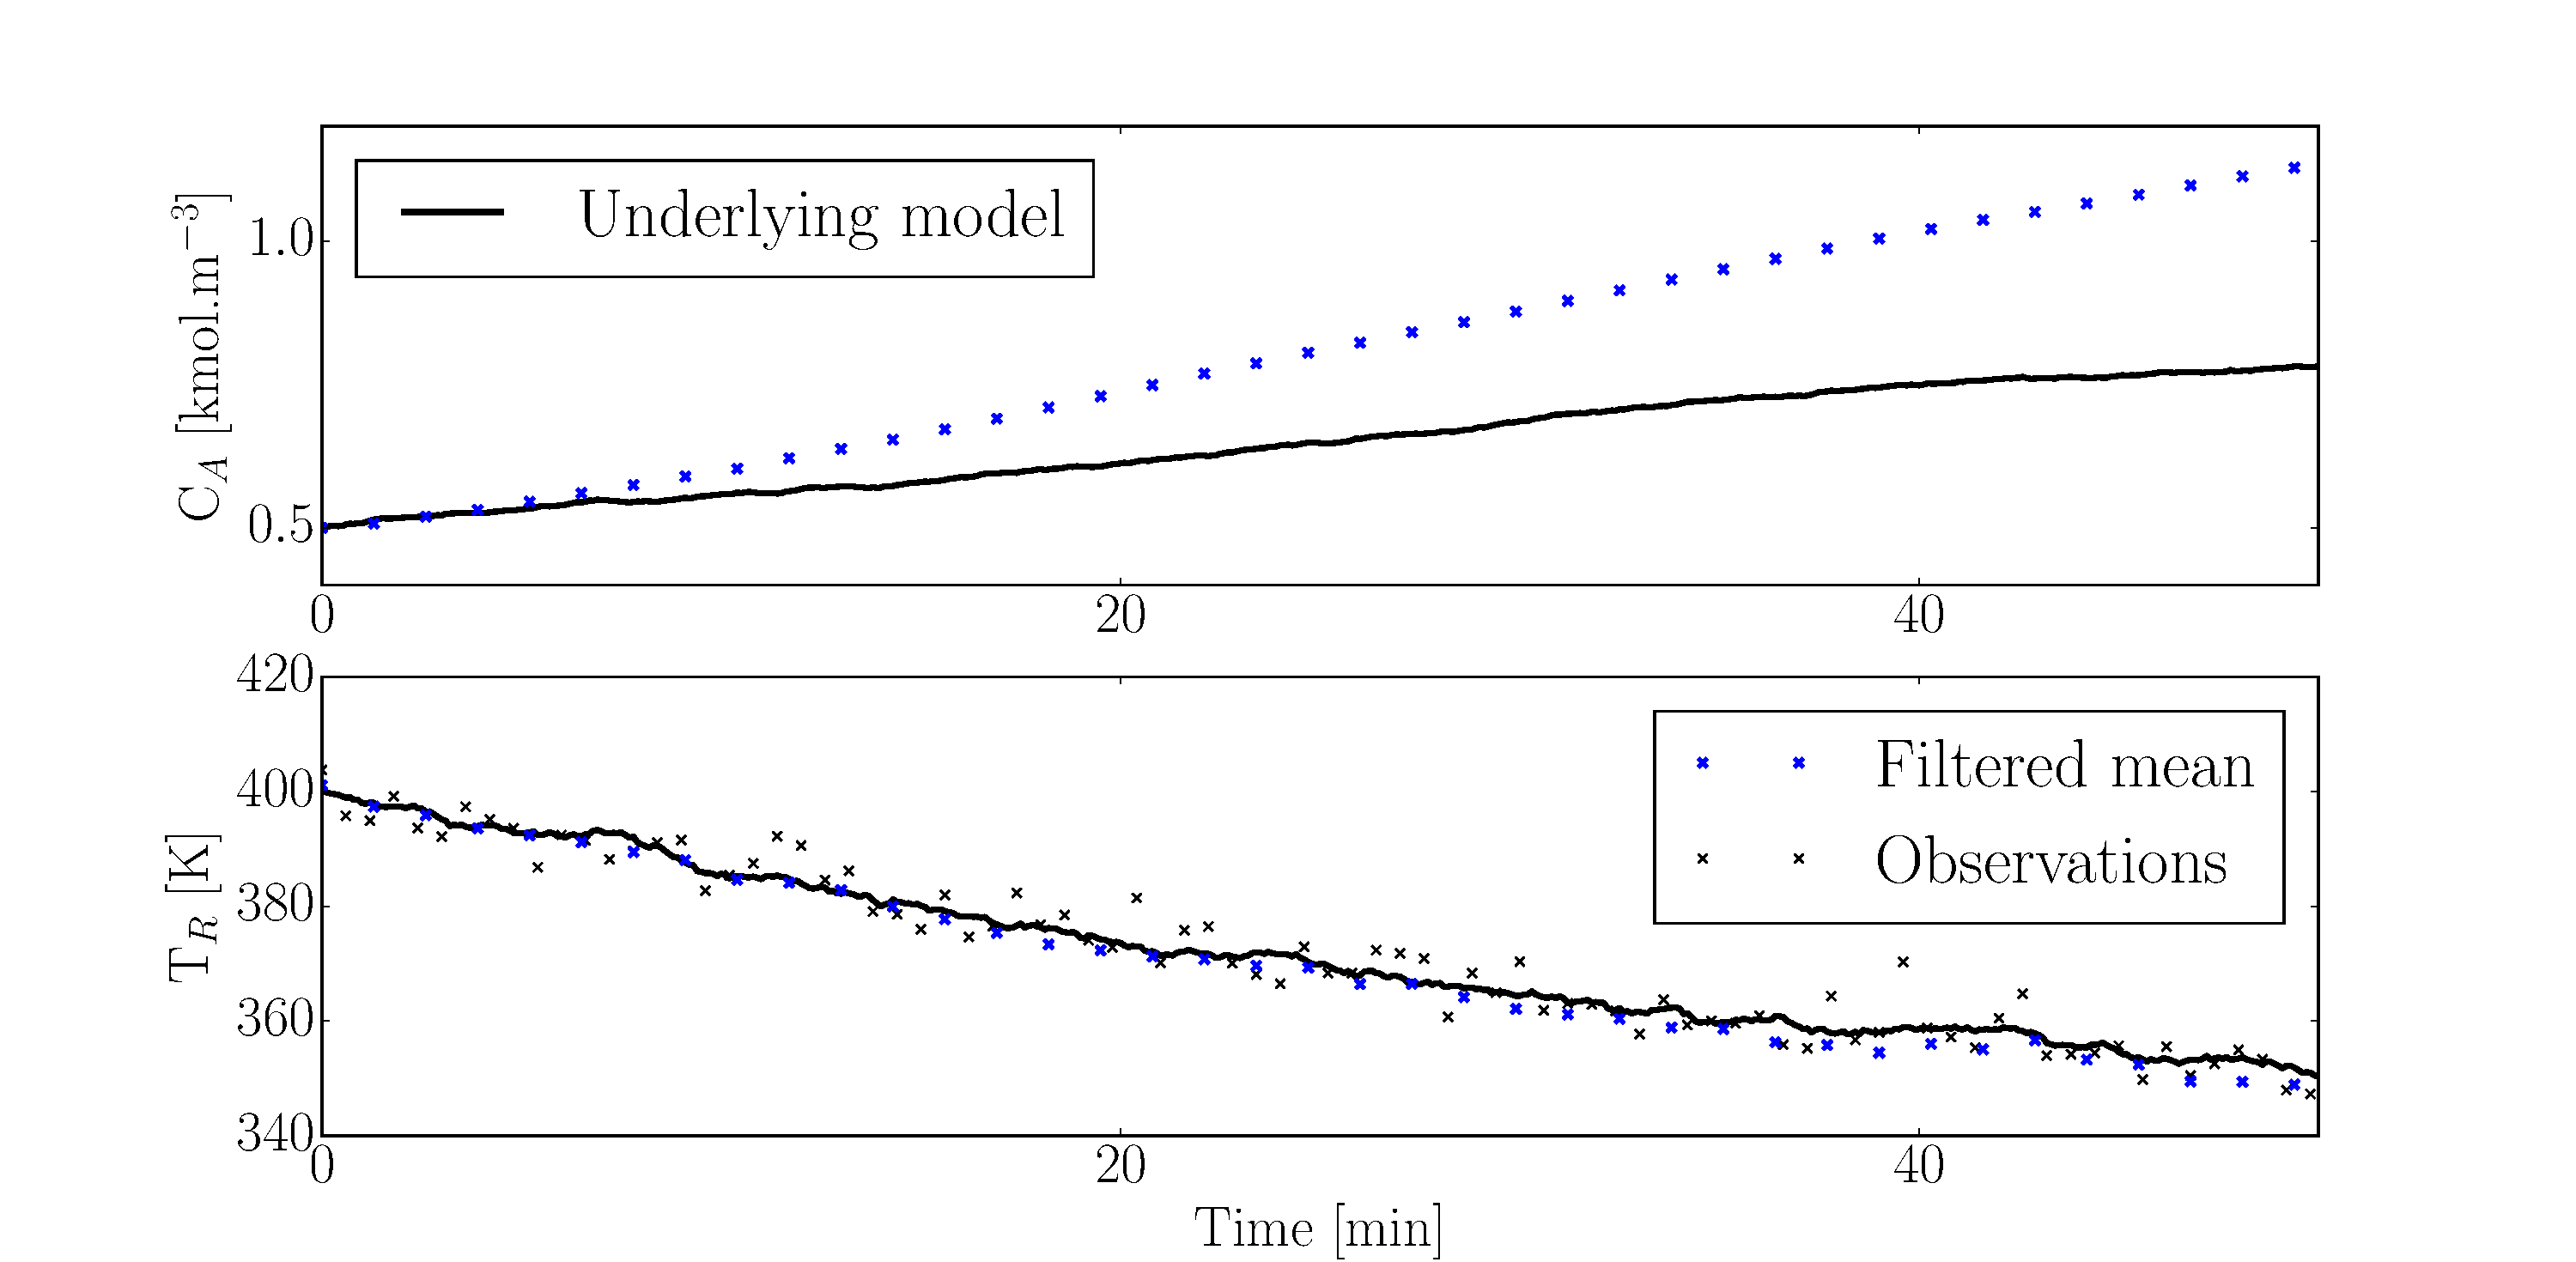
\includegraphics[width=\textwidth]{kalman_filter_timeseries_M1.pdf}
\caption{Kalman filter superimposed on the time series evolution of the CSTR with initial condition $(0.50, 400)$ and measuring only temperature.}
\label{fig_kftimeseries}
\end{figure}
In figure \ref{fig_kfphase} we see another interesting property of Kalman filters. The posterior covariance quickly converges to a constant value (the confidence region quickly stops changing shape/size) which is independent of the observations. This is a general property of linear Gaussian systems \cite{barber} and is evident from the recursion expression. The modelled system dynamics and noise are the only factors affecting the covariance. If the model is accurate this is not a problem but we see that as the model becomes less accurate the filter maintains the same level of confidence in its estimate. This is quite undesirable behaviour because the confidence in the estimate is not a function of the observations. 

It is also interesting to consider the shape of the confidence region. Notice that it is short vertically - indicating less uncertainty in the temperature state dimension but wide horizontally - indicating more uncertainty in the concentration state dimension. Intuitively this is plausible because, since we do not measure concentration, we are less sure about the underlying state. 

In figure \ref{fig_kfphase} we see that while the temperature estimate is still trustworthy (the temperature mean estimate lines up horizontally with the true underlying state) the concentration estimate diverges.
\begin{figure}[H] 
\centering
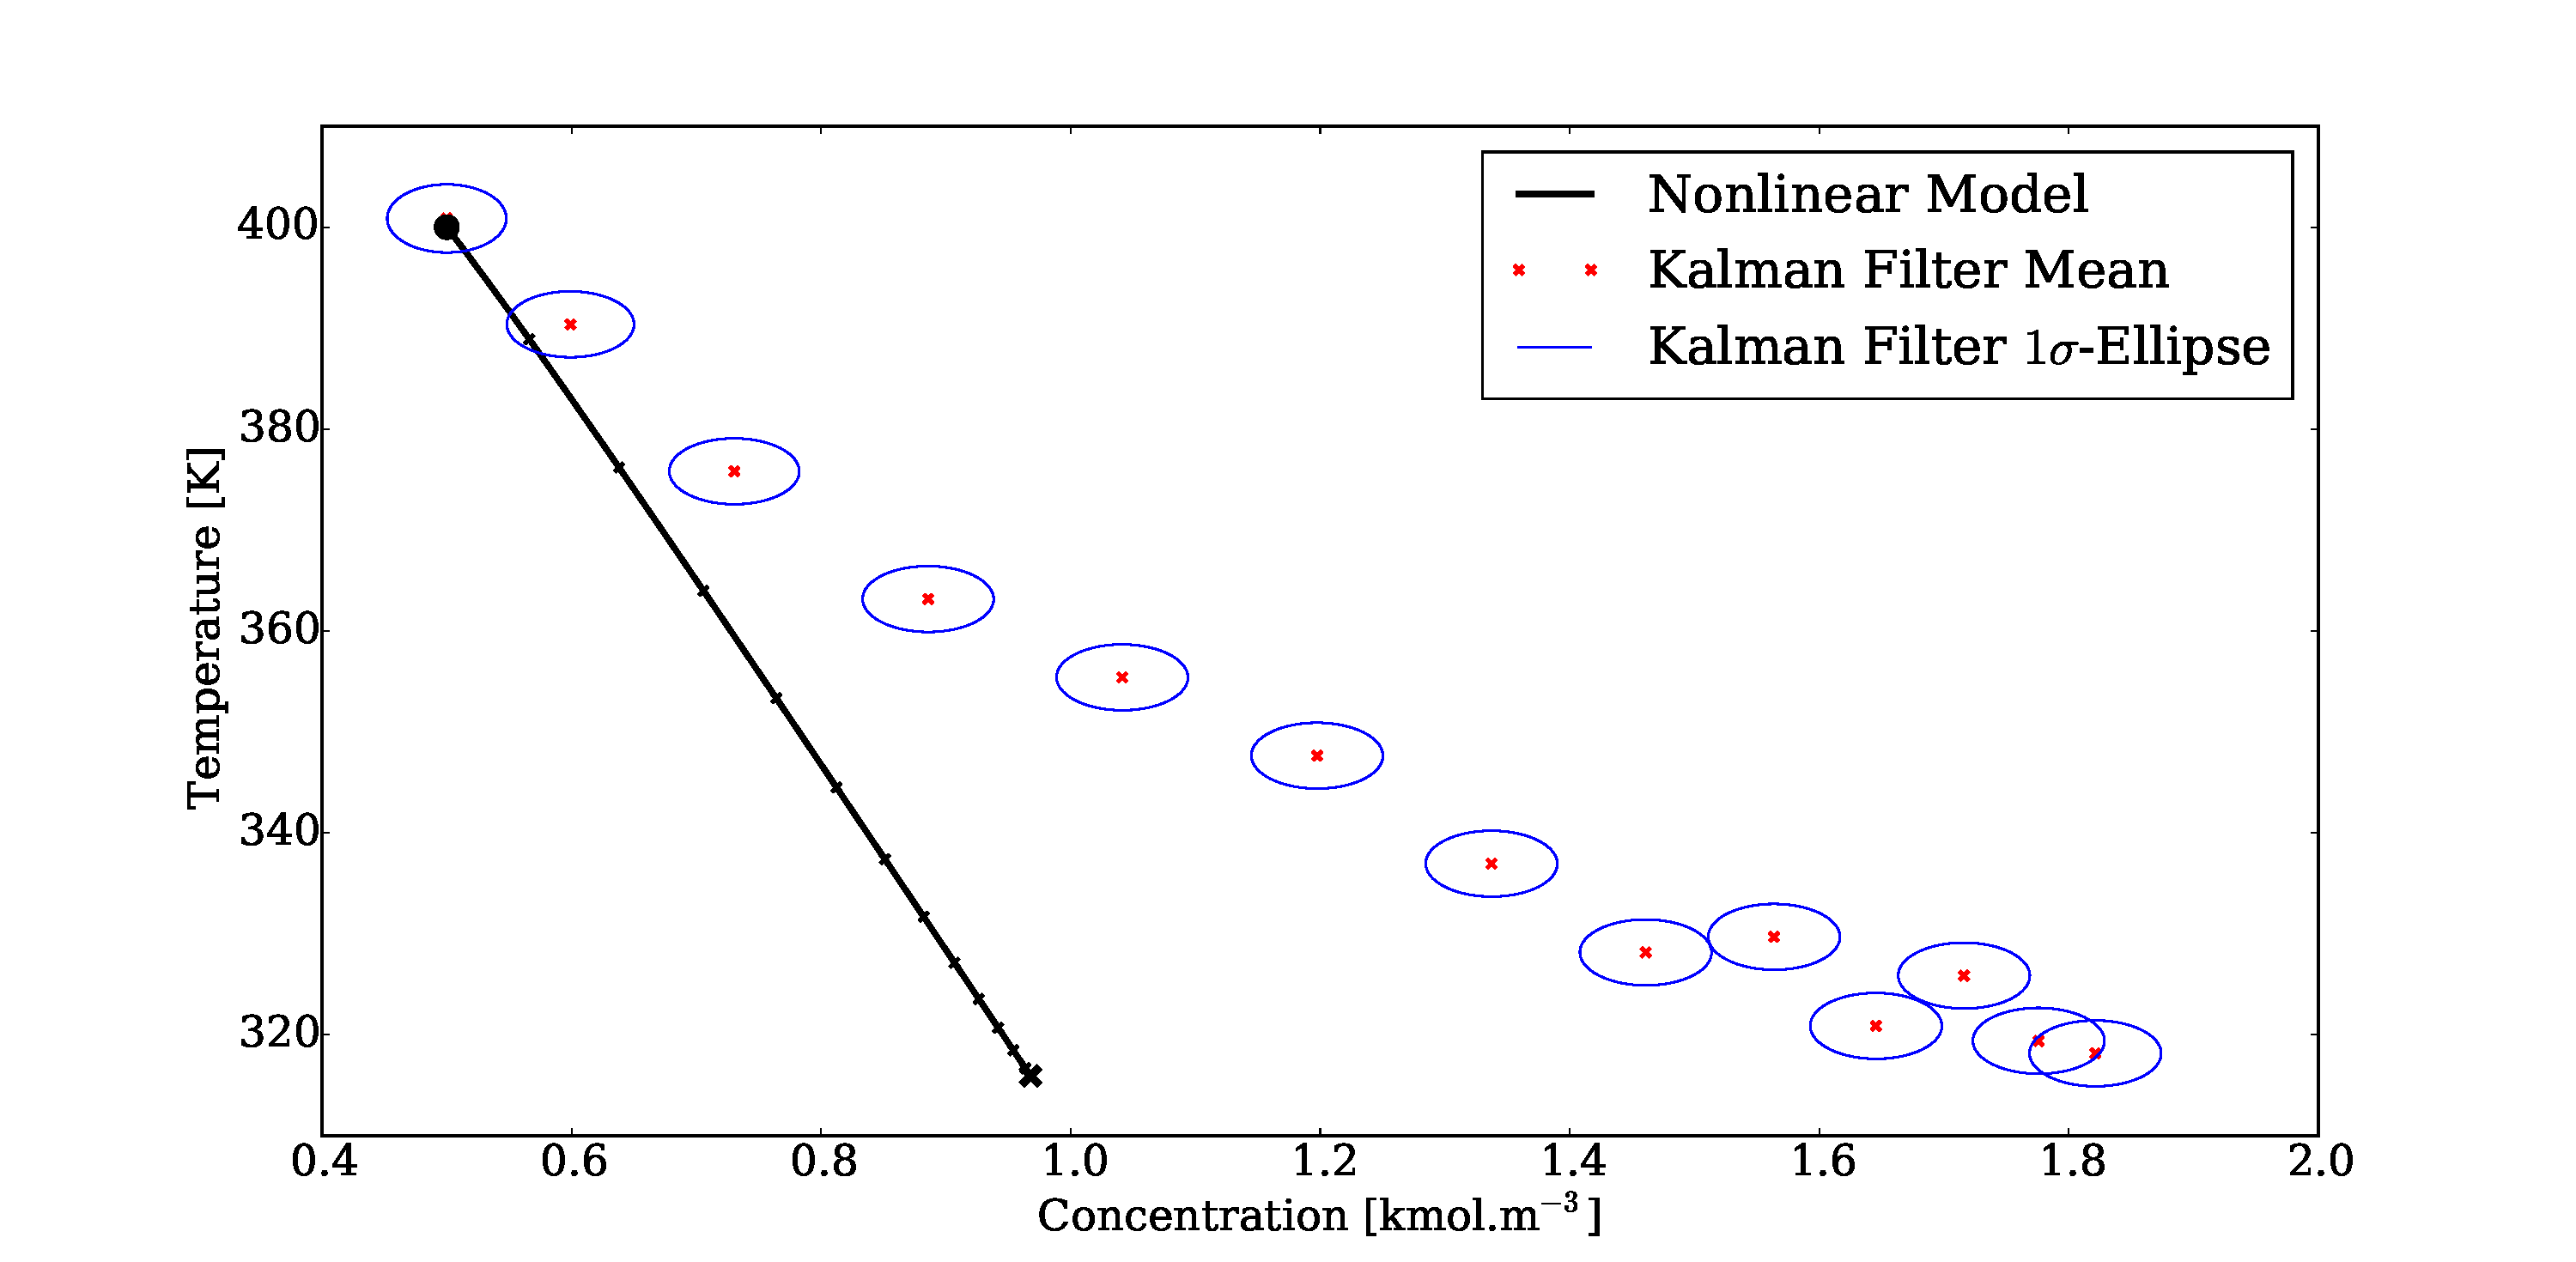
\includegraphics[width=\textwidth]{kalman_filter_phase_M1.pdf}
\caption{State space diagram of the CSTR with mean and 90\% confidence region superimposed thereupon. Only temperature is measured.}
\label{fig_kfphase}
\end{figure}
The root of the problem lies in the unsuitability of the model rather than our inference technique. It can be shown that for linear systems with Gaussian noise the Kalman filter is the optimal state estimator \cite{shalom}. 

Based on our discussion in chapter \ref{sec_cstr}, where the CSTR example was introduced, we know that the linear models will not be accurate in regions far removed from their linearisation points. We therefore modify (\ref{eq_linmodel}) to also incorporate concentration measurements to offset this weakness. In this case we have that $C = \begin{pmatrix}
1 & 0\\0 &1
\end{pmatrix}$ and $V = \begin{pmatrix}
1\times 10^{-3} & 0\\0 & 10
\end{pmatrix}$ with everything else the same. The time evolution of the states is shown in figure \ref{fig_kftime2} and the state space representation is shown in figure \ref{fig_kfphase2}. 
\begin{figure}[H] 
\centering
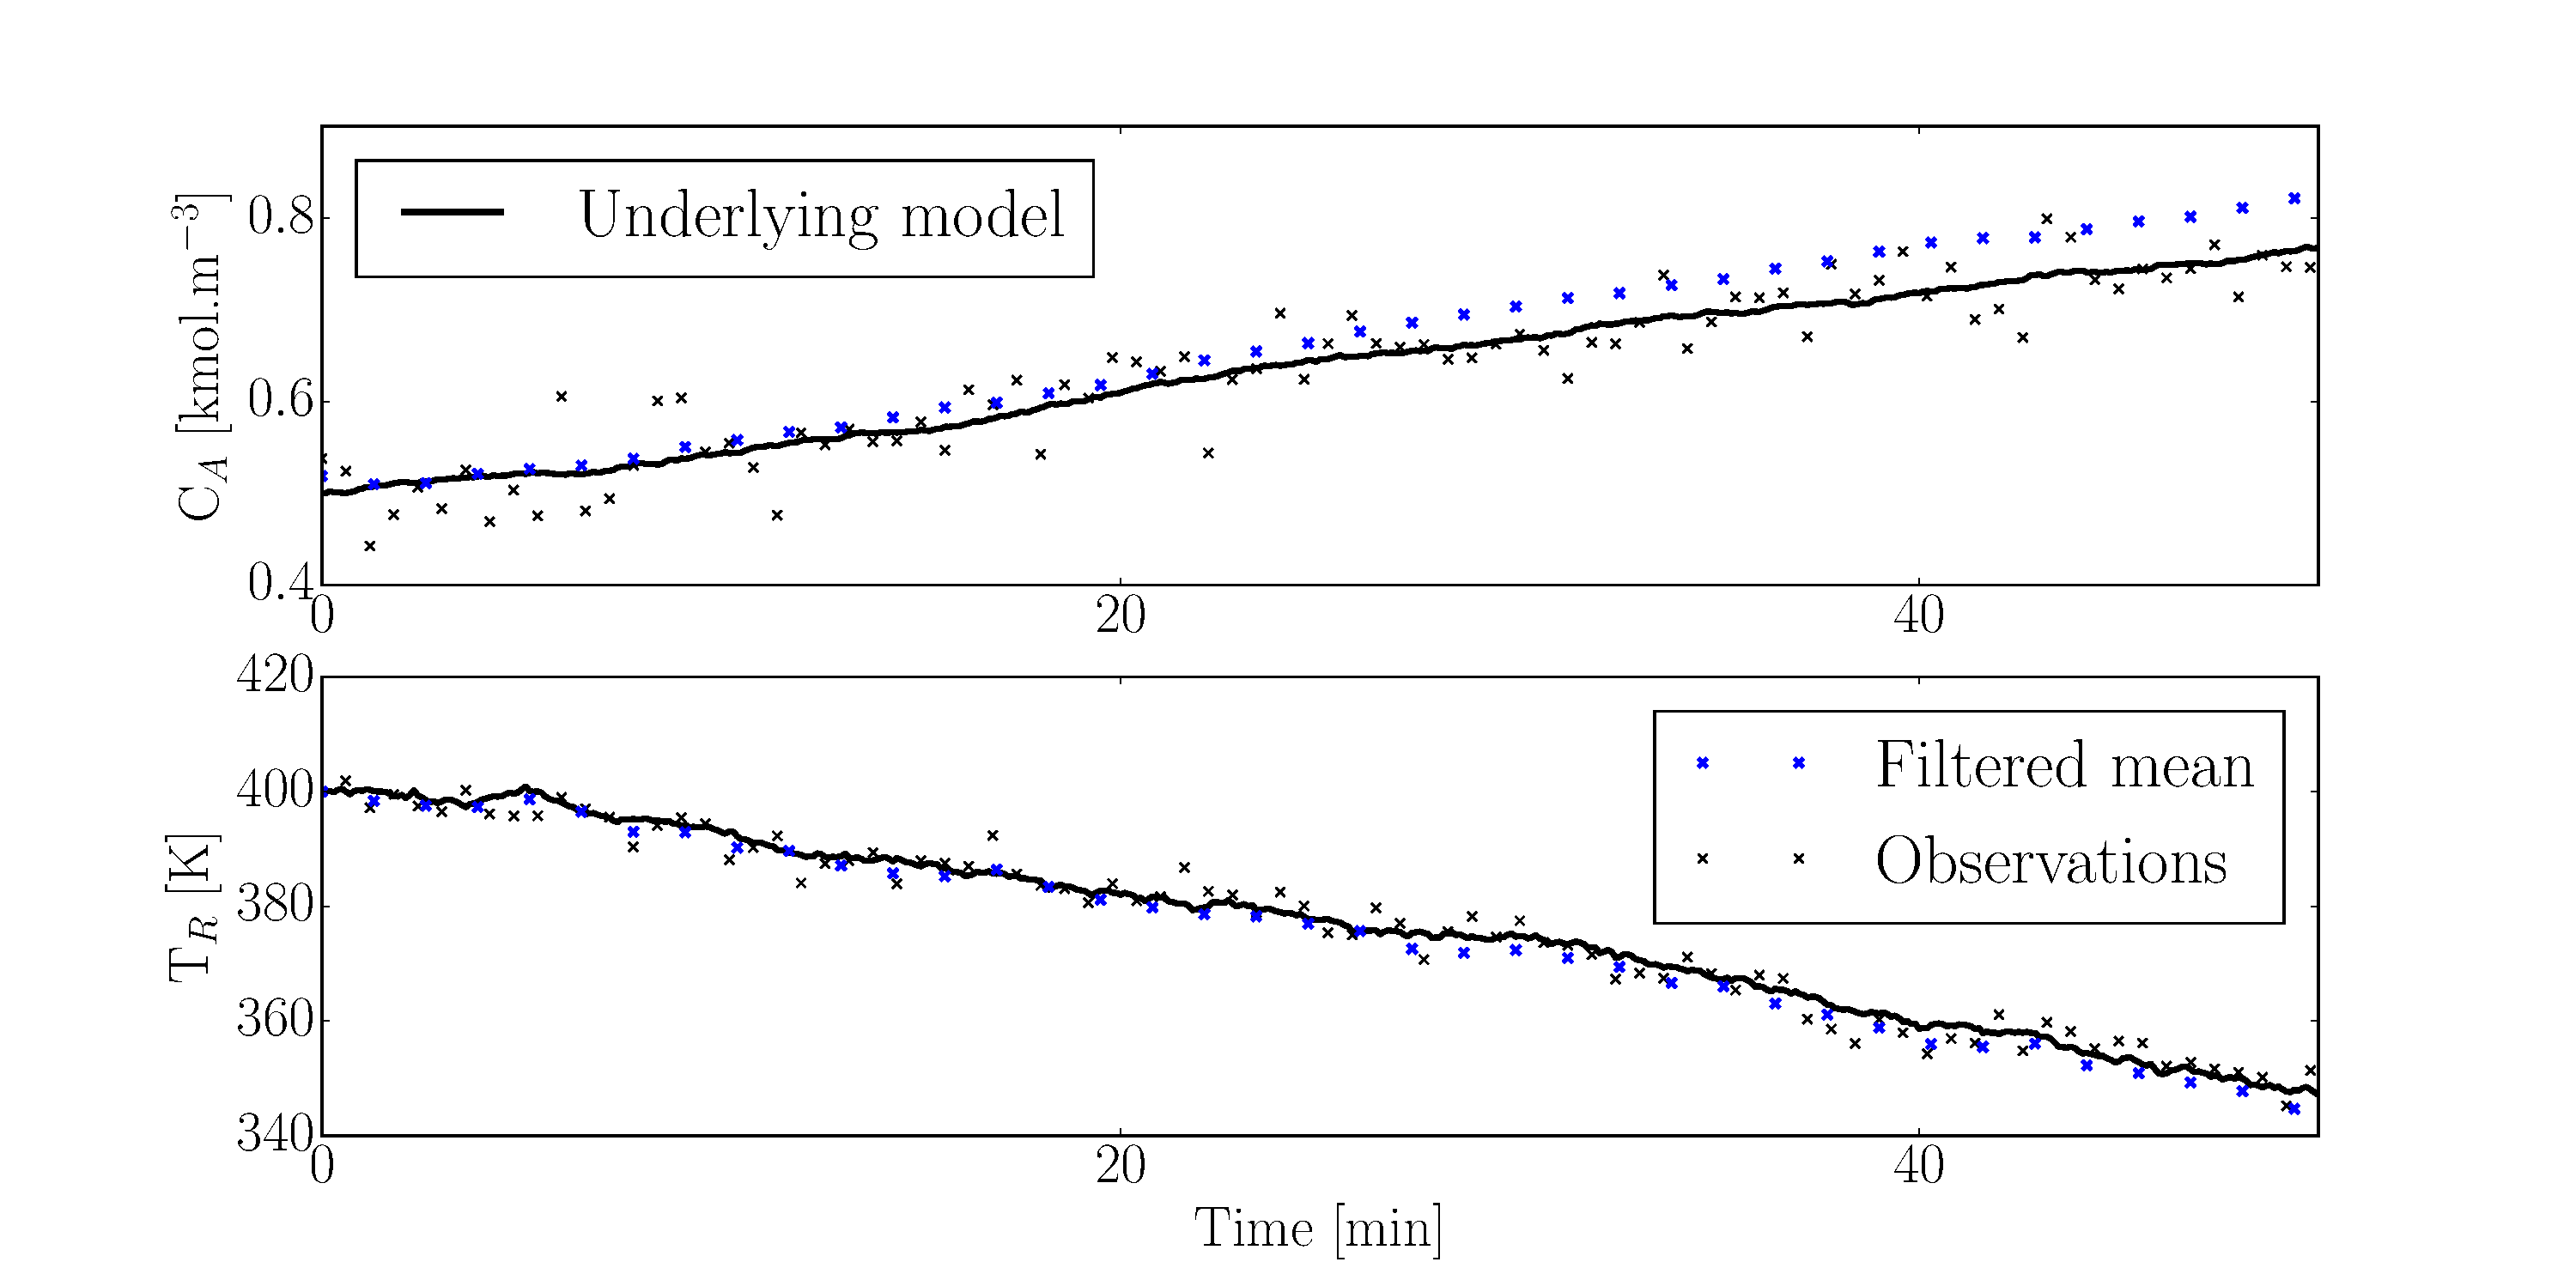
\includegraphics[width=\textwidth]{kalman_filter_timeseries_M2.pdf}
\caption{Kalman filter superimposed on the time series evolution of the CSTR with initial condition $(0.50, 400)$ and measuring both temperature and concentration.}
\label{fig_kftime2}
\end{figure}
\begin{figure}[H] 
\centering
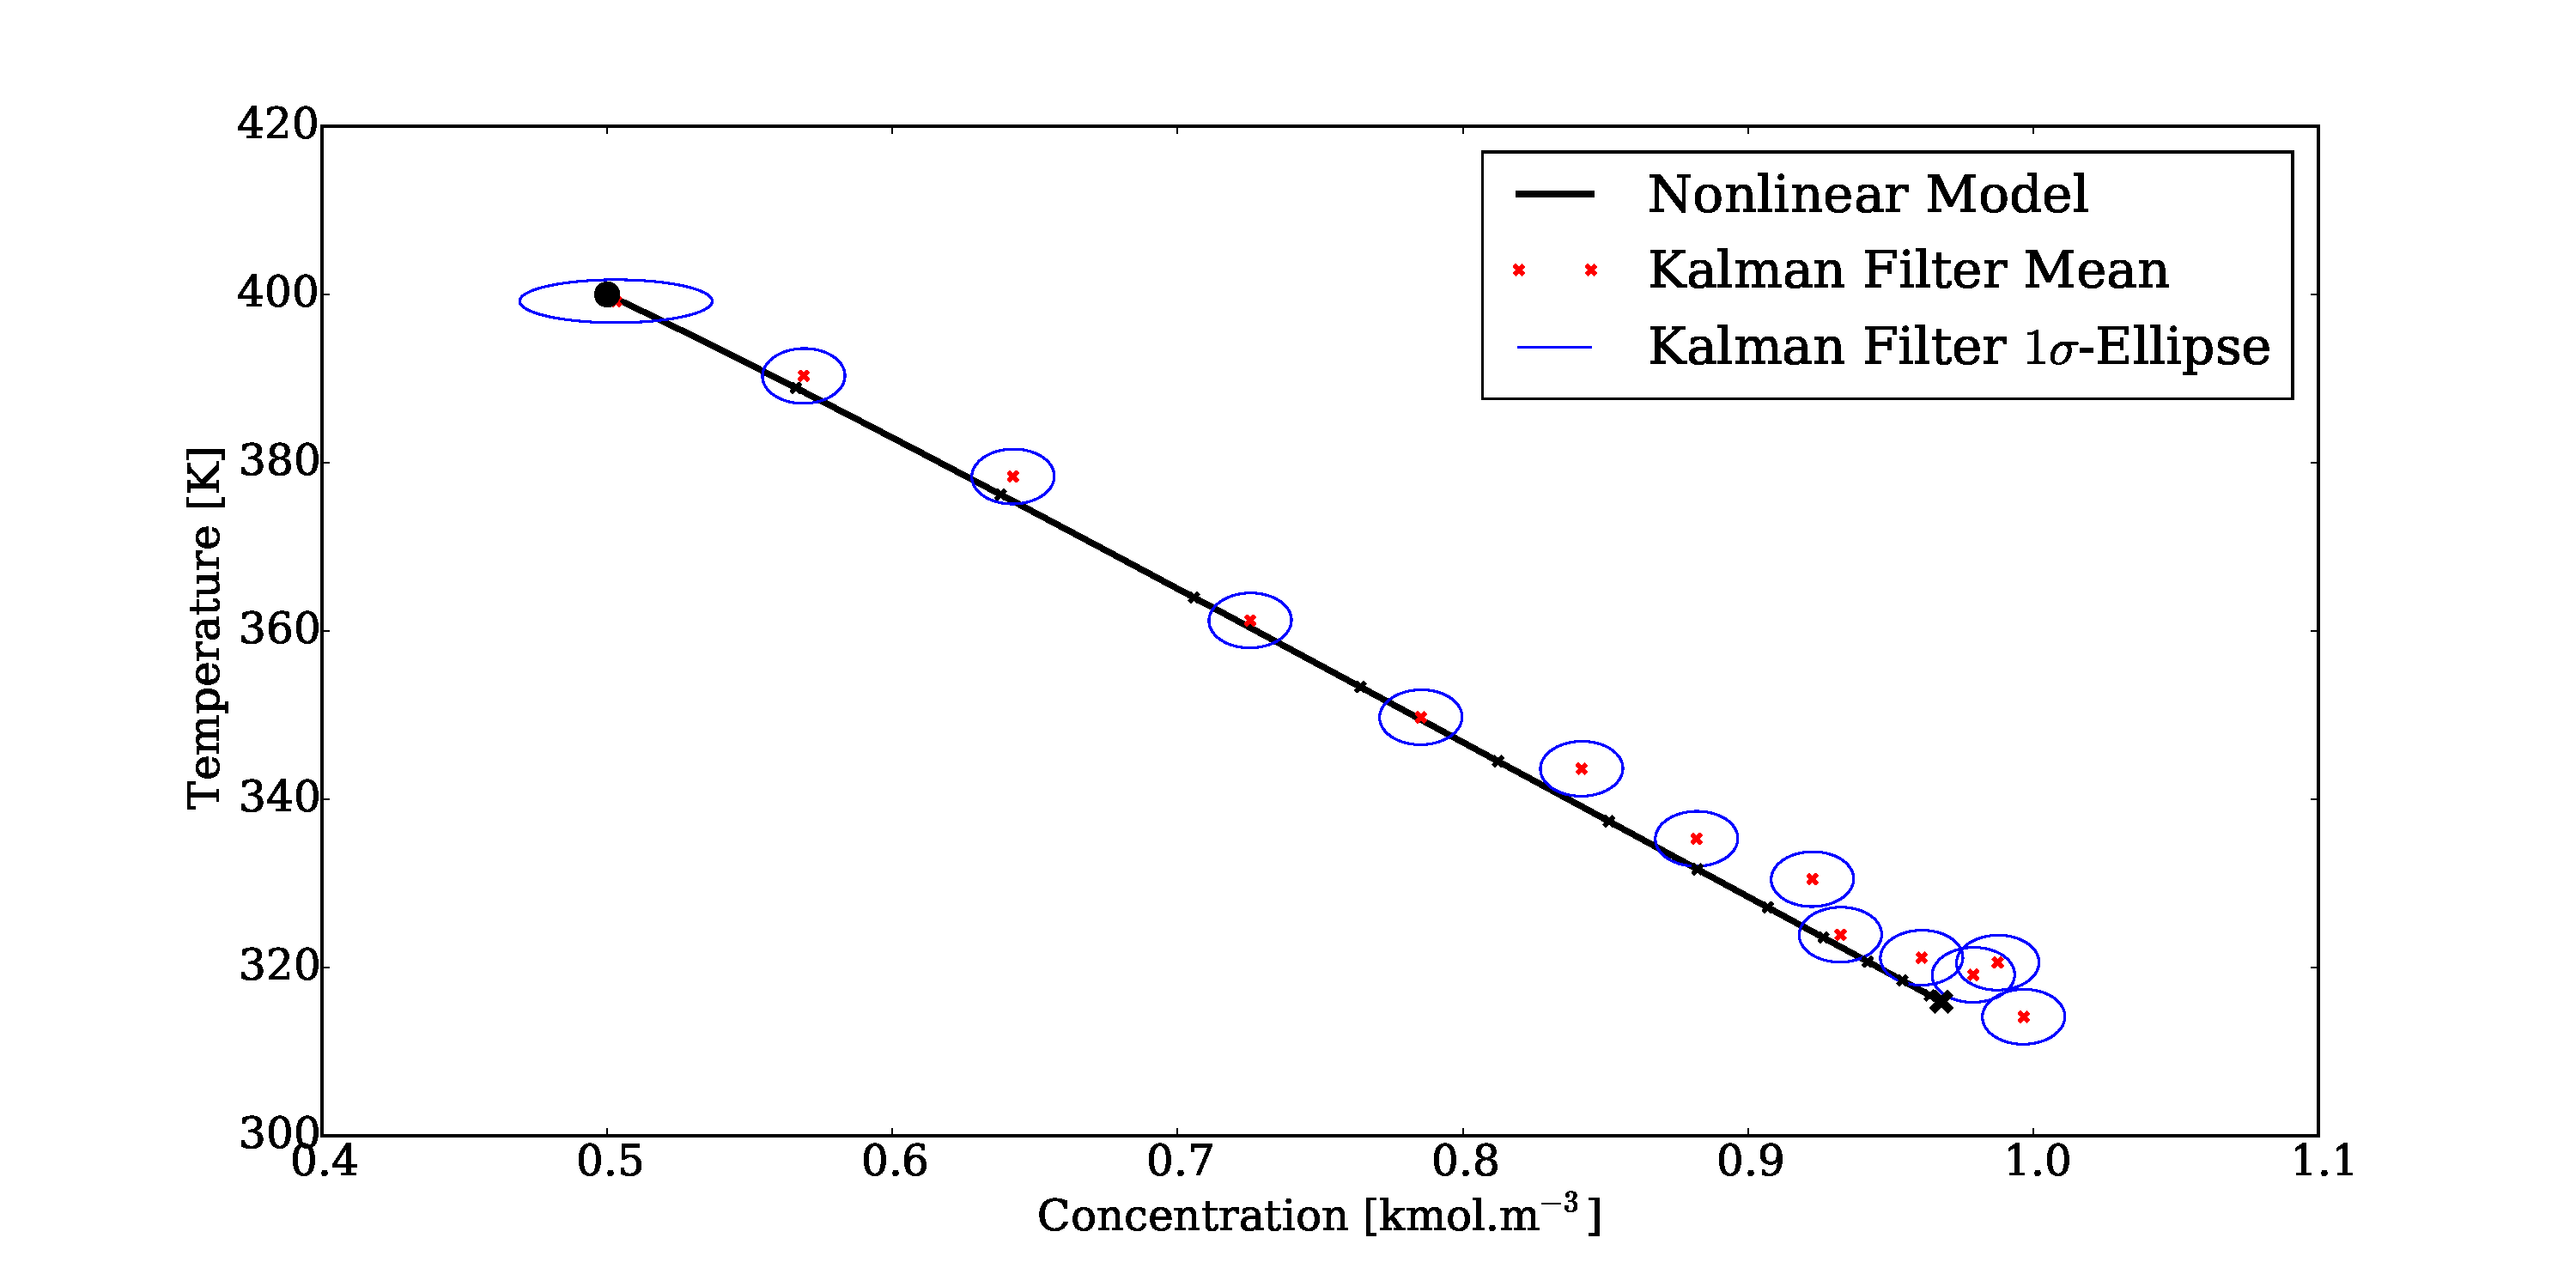
\includegraphics[width=\textwidth]{kalman_filter_phase_M2.pdf}
\caption{State space diagram of the CSTR with mean and 90\% confidence region superimposed thereupon. Both concentration and temperature are measured.}
\label{fig_kfphase2}
\end{figure}
Comparing figures \ref{fig_kfphase} and \ref{fig_kfphase2} we see that by incorporating the state measurement the state estimation is much more accurate. The average concentration and temperature estimation error is only 4.09\% and 0.45\% respectively. It is not necessary to directly measure concentration as we have done: any measurement which depends on $C_A$ (or even both $C_A$ and $T_R$) would suffice. The second measurement reduces our uncertainty in the concentration state estimate because we have more to base our inference on than just a bad model.  

In the next chapter we drop the linearity and normality assumptions at the cost of the closed form, exact inference solutions. Sections \ref{sec_kalman_filter_deriv} and \ref{sec_lin_prediction} form the basis of chapter \ref{sec_linear_control} and we encourage the reader to familiarise themselves with it. 